\section{Proxy Based Firewall}
Als Nachteil der ``\nameref{sec:packet-filter-firewall}'' wird erwähnt, dass lediglich der Inhalt des IP-Headers im Zuge der Überprüfung analysiert wird.

Die \emph{Proxy Based Firewall} fügt der ``\nameref{sec:packet-filter-firewall}'' spezifische Applikations-Proxies hinzu, welche den eingehenden Traffic überprüfen und ggf. an den internen, eigentlichen Dienst weiterleiten.

Der interne Dienst wird auf diese Weise für den externen Host  komplett unsichtbar; er kommuniziert lediglich mit dem Proxy.


\subsection*{Kontext}
Netzwerkverkehr soll auf der Ebene des Application-Layers gefiltert werden können (vgl. ``\nameref{sec:packet-filter-firewall}'' tut dies lediglich auf dem Network-Layer). Auf diese Weise soll sichergestellt werden, dass keine schädlichen Befehl/schädlicher Code ins eigene Netz hinein gelangt resp. aus dem eigenen Netz heraus gesendet werden kann (Würmer, Trojaner etc.).

\subsection*{Problem}
Wie kann die ``\nameref{sec:packet-filter-firewall}'' so erweitert werden, dass nicht nur der IP-Header zur Filterung von Netzwerkverkehr verwendet werden kann? Wie kann auch der IP-Payload in die Filterung miteinbezogen werden?

Ergänzend zu den bei der \nameref{sec:packet-filter-firewall} definierten Forces kommen folgende neu hinzu:

\begin{itemize}
	\item In unserem Netzwerk werden verschiedenste Dienste angeboten. Entsprechend Umfangreich muss auch das Wissen der Firewall über die jeweiligen Dienste sein.
\end{itemize}


\subsection*{Lösung}

\begin{figure}[H]
	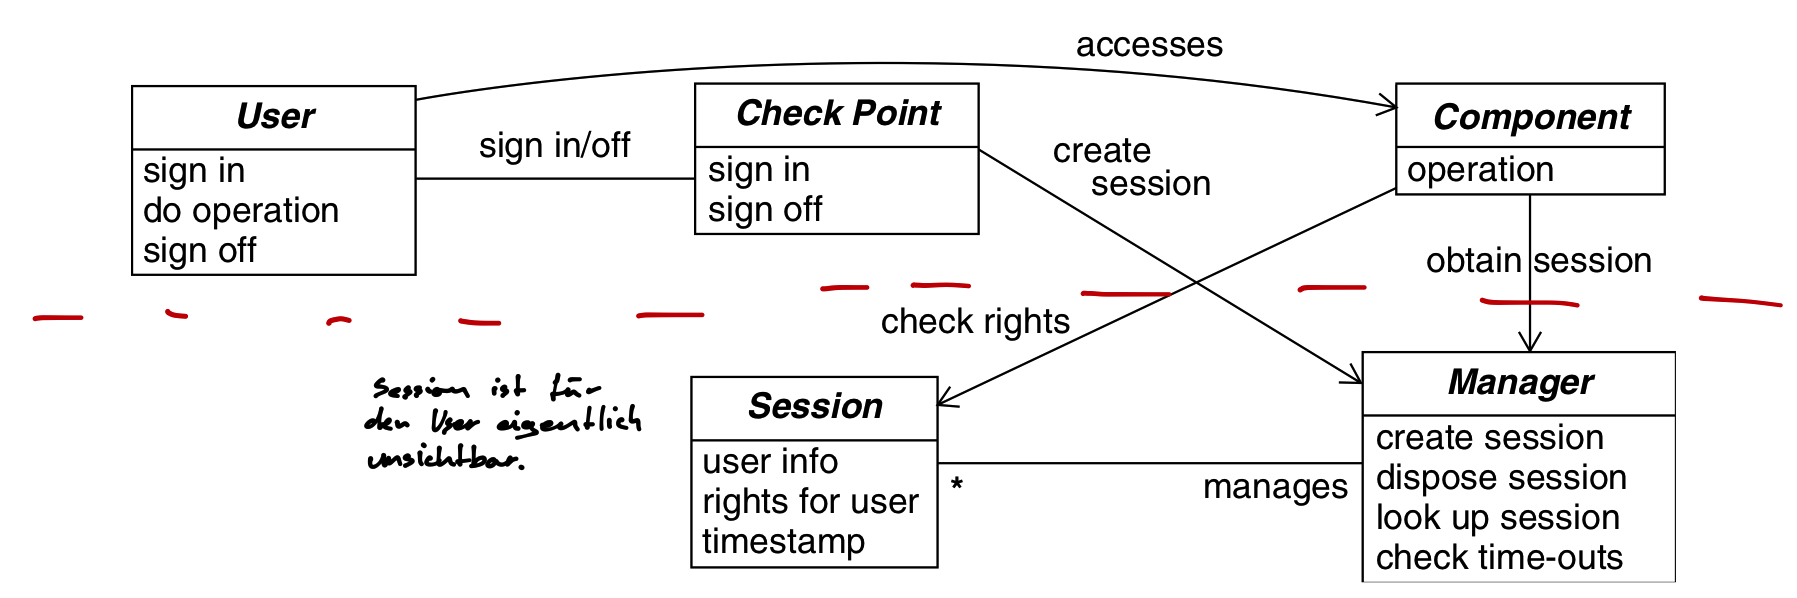
\includegraphics[width=\textwidth]{content/system-access-control-architecture/images/security-session-structure.png}
	\caption{Security Session: Schematischer Aufbau \cite{SecPatterns06}}
\end{figure}


\subsubsection*{Implementierung}
\begin{enumerate}
	\item 
\end{enumerate}


\subsection*{Vorteile}
\begin{itemize}
	\item 
\end{itemize}


\subsection*{Nachteile}
\begin{itemize}
	\item 
\end{itemize}


\subsection*{Reallife Beispiele}
\begin{itemize}
	\item 
\end{itemize}


\subsection*{Mögliche Prüfungsfragen}
\begin{itemize}
	\item 
\end{itemize}